\section{Models and different Approaches}
\subsection{Challenges}

We dedicated time to understand how the openai-gym is working internally. For this specific problem, we understood how the rewards and environment is behaving on every episode, as described in infrastructure. Moreover, to get faster results, we focused on better machine and GPU settings on google cloud and getting docker environment setup for codalab and reproducibility across platforms.

\subsection{Modelling the problem}

Basic framework is defined in Fig 1. The agent performs action($a$) on the environment. Performing the action on the environment returns reward($r$) and new state $s'$. Our agent then incorporates this information.

\begin{figure}[!ht]
%\begin{figure}%
%\vspace*{\fill}
\centering
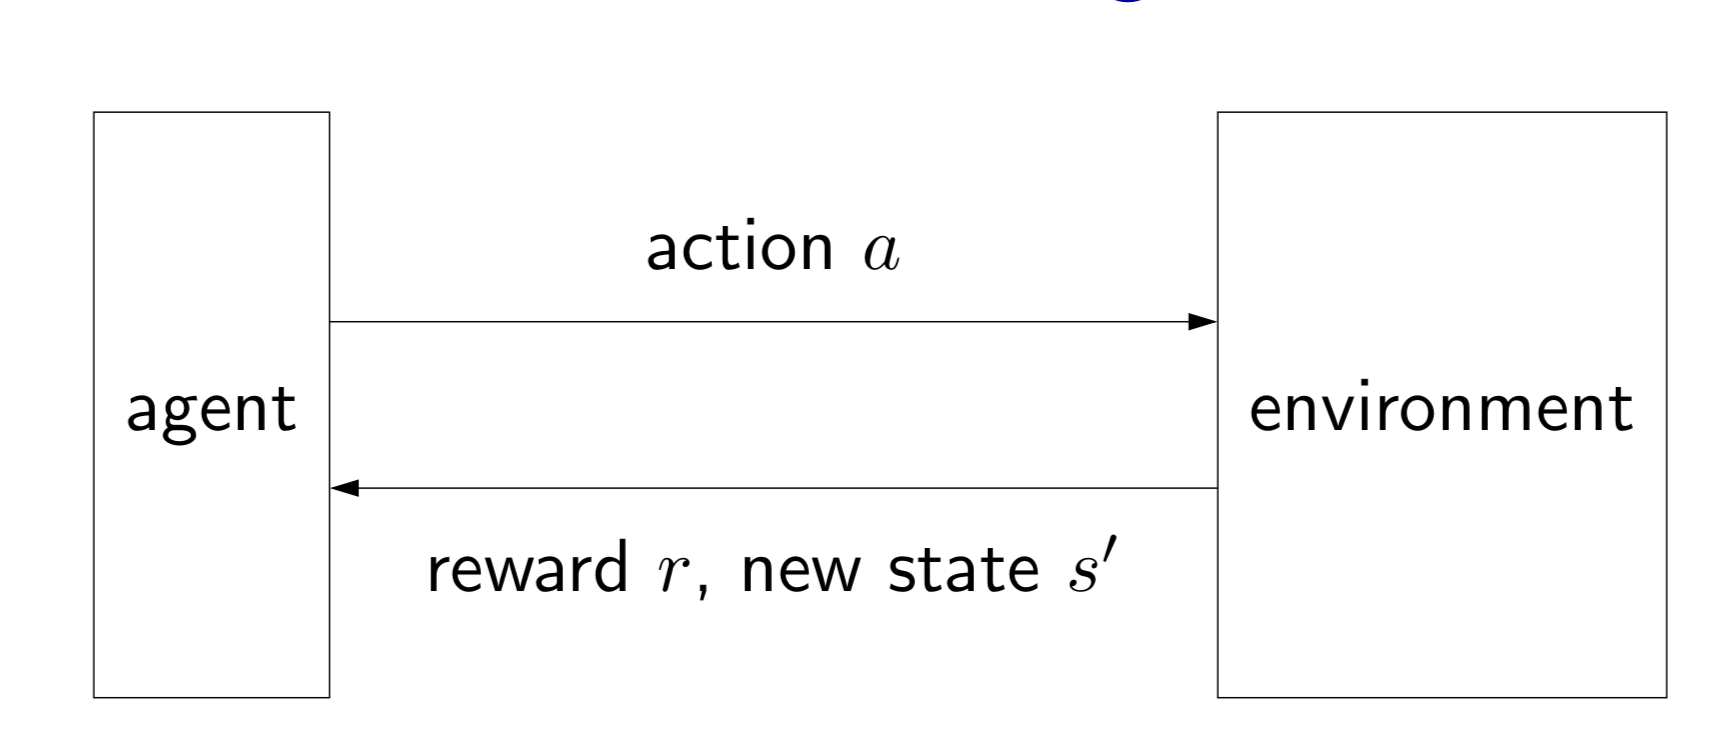
\includegraphics[scale=0.25,width=0.25\columnwidth]{reinforcement_framework.png}%
\caption{ Reinforcement Learning Framework}%
\label{fig:Visualization}%
\end{figure}
%\vfill}

In such a model, for our problem, here is quick description of notations:
\begin{enumerate}
\item $S$ is defined as all possible states, $s$ is one particular 8 dimensional state
\item $A$ is defined as all possible actions, $a$ is one of the actions out of $[\text{idle}, \text{fire engine}, \text{rotate left}, \text{rotate right}]$
\item $R$ is the reward distribution given $(s, a)$
\item $P$ is the set of possible transitions and their probabilities given $(s, a)$
\item $\gamma$: the discount factor. How much we want our agent to discount future reward. It is a hyperparameter that we define ourselves.
\end{enumerate}

Our model builds off of Q-learning algorithms by using a Deep Neural Network (DNN) for approximating the state-action Q-value, Q(s, a). 
Given the state $s$, our goal is to identify a policy $\pi_{opt}$ that maps the states to actions in order to maximize the total reward we get.

\begin{center}
S $\rightarrow$ A based on $\pi_{opt}$
\end{center}

As we know, $Q$ value is defined as the expected reward that we get following action $a$ in a given state $s$ and then following the policy $\pi$, our objective is to define a $Q_{opt} (s, a)$, which can be maximised over all possible actions at a state $s$, in order to find the $\pi_{opt}$.

\subsection{Algorithms and Equations}

\subsubsection{DQN Introduction}

Model-free based Deep Q Network algorithm was chosen specifically for the state size and complexity. DQN builds off of Q-learning algorithms by using a Deep Neural Network (DNN) for approximating the state-action value function, Q(s, a). Function Q(s, a) is defined such that for given state $s$ and action $a$ it returns an estimate of a total reward we would achieve starting at this state, taking the action and then following some policy. Let’s call the Q function for the optimal policies $Q_{opt}$.
 $Q_{opt}$ with discounting can be written as 
 \begin{equation}
Q_{opt}(s,a) = r_{0} + \gamma r_{1} + \gamma^{2} r_{2} + ...
\end{equation}
Here, $r$ stands for rewards. $\gamma$ is called a discount factor and when set it to $\gamma < $  1 , it makes sure that the sum in the formula is finite. The $\gamma$ controls how much the function Q in state $s$ depends on the future and so it can be thought of as how much ahead the agent sees.  \newline
The above equation can be rewritten in a recursive form.
 \begin{equation}
Q_{opt}(s,a) = r_{0} + \gamma max_{a}Q_{opt}(s',a)
\end{equation}
This equation is proven to converge to the desired $Q_{opt}$, with finite number of states and each of the state-action pair is presented repeatedly. However, the Lunar Lander state space is real and continuous. We cannot store infinite number of values for every possible state. Instead, we  approximate the Q function with a neural network. This network will take a state as an input and produce an estimation of the Q function for each action. This network with multiple layers is called Deep Q-network (DQN).
\newline \newline
\textbf{Experience Replay} \newline \newline
During each simulation step, the agent perform an action $a$ in state $s$, receives immediate reward $r$ and come to a new state $s’$.
\newline
There are two problems with online learning - \newline
1. The samples arrive in order they are experienced and as such are highly correlated. This might cause overfitting.
\newline
2. Throwing away each sample immediately after we use it. This means we are not using our experience effectively.
\newline
The key idea of 'experience replay' is that we store these $(s, a, r, s')$ transitions in a memory and during each learning step, sample a random batch and perform a gradient descend on it. This way we solve both issues.
After reaching the finite allotted memory capacity, the oldest sample is discarded.
\newline \newline
\textbf{Exploration}
To find out that actions which might be better then others, we use $\epsilon$ greedy policy. This policy behaves greedily most of the time, but chooses a random action with probability $\epsilon$. $\epsilon$ will be a hyper-parameter played with to make sure our agent learns fast enough while consistently performing better.

\subsubsection{Full DQN}
In DQN algorithm we set targets for gradient descend as:
\begin{equation}
Q_{opt}(s,a) = r_{0} + \gamma max_{a}Q_{opt}(s',a)
\end{equation}
We see that the target depends on the current network. A neural network works as a whole, and so each update to a point in the Q function also influences whole area around that point. And the points of $Q(s, a)$ and $Q(s’, a)$ are very close together, because each sample describes a transition from $s$ to $s’$. This leads to a problem that with each update, the target is likely to shift. This can lead to instabilities, oscillations or divergence.
\newline
\begin{figure}[!ht]
%\begin{figure}%
%\vspace*{\fill}
\centering
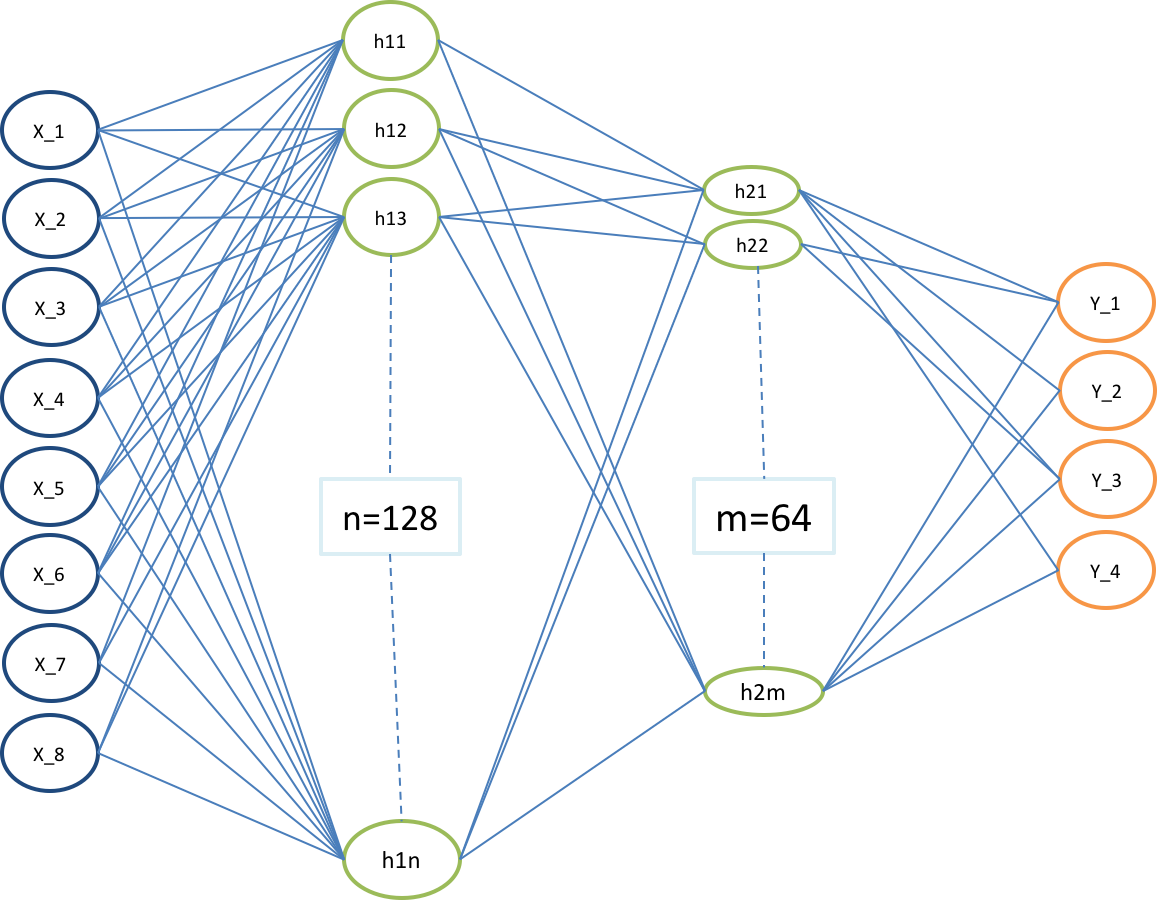
\includegraphics[scale=0.35,width=0.35\columnwidth]{figures/NN.png}%
\caption{ DQN with two layers used to model the agent}%
\label{fig:Visualization}%
\end{figure}
%\vfill}

To overcome this problem, researches proposed to use a separate target network for setting the targets. This network is a mere copy of the previous network, but frozen in time. It provides stable $\tilde{Q}$ values and allows the algorithm to converge to the specified target:
\begin{equation}
Q(s, a) \xrightarrow{} r + \gamma max_a \tilde{Q}(s', a)
\end{equation}

After several steps, the target network is updated, just by copying the weights from the current network. To be effective, the interval between updates has to be large enough to leave enough time for the original network to converge. \newline
For lunar lander, we update target model after every episode.

\subsubsection{Double DQN}
One problem in the DQN algorithm is that the agent tends to overestimate the Q function value, due to the max in the formula used to set targets.
Because of the max in the formula, the action with the highest positive/negative error could be selected and this value might subsequently propagate further to other states. This leads to bias – value overestimation. This severe impact on stability of the learning algorithm.
\newline
In this new algorithm, two Q functions $Q_{1}$ and $Q_2$ – are independently learned. One function is then used to determine the maximizing action and second to estimate its value. Either $Q_1$ or $Q_2$ is updated randomly with a formula:
\begin{equation}
Q_1(s, a) \xrightarrow{} r + \gamma Q_2(s', argmax_a Q_1(s', a)) 
\end{equation}
or
\begin{equation}
Q_2(s, a) \xrightarrow{} r + \gamma Q_1(s', argmax_a Q_2(s', a)) 
\end{equation}
It was proven that by decoupling the maximizing action from its value in this way, one can indeed eliminate the maximization bias.
\newline
When thinking about implementation into the DQN algorithm, we can leverage the fact that we already have two different networks giving us two different estimates Q and $\tilde{Q}$ (target network). Although not really independent, it allows us to change our algorithm in a really simple way.
\newline
The original target formula would change to:
\begin{equation}
Q(s, a) \xrightarrow{} r + \gamma \tilde{Q}(s', argmax_a Q(s', a))
\end{equation}
We could observe that Double DQN was more stable than Full DQN.
 
\subsubsection{Dueling layer DQN}
Q(s,a) represents the value of a given action $a$ chosen in state $s$, V(s) represents the value of the state independent of action. By definition, $V(s)=max_{a}Q(s,a)$. Thus, A(s,a) provides a relative measure of the utility of actions in s. The insight behind the dueling network architecture is that sometimes the exact choice of action does not matter so much, and so the state could be more explicitly modeled, independent of the action. There are two neural networks — one learns to provide an estimate of the value at every timestep, and the other calculates potential advantages of each action, and the two are combined for a single action-advantage Q function. We can achieve more robust estimates of state value by decoupling it from the necessity of being attached to specific actions.FIXME%\citep{Dueling}
\newline
\begin{equation}
Q(s,a) \rightarrow A(s,a) + V(s)
\end{equation}
The above equation is unidentifiable in the sense that given $Q$
we cannot recover $V$ and $A$ uniquely. This lack of identifiability is mirrored by poor practical performance when this equation is used directly. To address this issue of identifiability, we can force the advantage
function estimator to have zero advantage at the
chosen action. That is, we let the last module of the network
implement the forward mapping.
\begin{equation}
Q(s,a; \theta, \alpha, \beta) \rightarrow V(s; \theta, \beta) + (A(s,a\theta, \alpha) - max_{a' \epsilon |A|} A(s,a';\theta,\alpha ))
\end{equation}
An alternative module replaces the max operator with an
average. On the one hand this loses the original semantics of V and
A because they are now off-target by a constant, but on
the other hand it increases the stability of the optimization:
with this following equation-
\begin{equation}
Q(s,a; \theta, \alpha, \beta) \rightarrow V(s; \theta, \beta) + (A(s,a\theta, \alpha) - \frac{1}{A} \sum_{a'}^{} A(s,a';\theta,\alpha ))
\end{equation}
 the advantages (A) only need to change as fast as the
mean, instead of having to compensate any change to the
optimal action’s advantage in  (13)
\newline
 
 \subsection{Accuracy and Efficiency Trade-off}

For our solutions, accuracy can be considered as consistency in getting more than 200 scores over a period of episodes. And efficiency would be how sooner we can get such weights for which the agent scores more than 200 scores. \\

When we train for more number of episodes (low efficiency), we get high accuracy (drop between consecutive episodes is lesser). And vice versa, if we stop early, we are highly efficient but accuracy is lower.

\subsection{Implementation choices}

The choice of state was based on the actual configuration of the lunar lander, and we learnt weights for each feature in the state. Another choice could have been training on image data, feeding images per episode and learning on gained rewards. Since this would have been computationally expensive, we chose the former approach to explicit definition of state space and learning it's weights. \\

For running different algorithms, we created separate classes so that the code is not only modularized, but can also be run easily on different openai environments, learning algorithms can be easily changed etc. Here's a quick description of different classes:

\begin{enumerate}
\item \textbf{Brain:} Class which contains keras models, updates the weights through train function and performs prediction based on learnt weights. 
\item \textbf{Memory:} Class which appends observations until maximum memory length and samples based on given batch size hyperparameter
\item \textbf{Agent:} Our agent class which explores and exploits based on fixed hyperparameters(gamma, epsilon max, epsilon min and decay) and passed arguments. This is also the class where we are performing the replay action and training the agent's brain instance. It also contains another instance of memory class which is used in replay while sampling.
\item \textbf{Environment:} Class which runs the episode on given agent and asks the agent to observe and replay whenever the agent is trying to learn on episodes. It returns the information on how much reward was observed on each episode and for how long each episode ran
\end{enumerate}
